\documentclass[12pt]{book}
\usepackage{hyperref}
\bibliographystyle{agsm}
\usepackage{har2nat}
\usepackage{amsmath,amssymb,amsthm,amscd,verbatim,graphicx,color}
\usepackage{enumitem}
\hypersetup{colorlinks=true, urlcolor=blue, citecolor=black, linkcolor=black}
\usepackage[x11names, rgb]{xcolor}
\usepackage[utf8]{inputenc}
%\usepackage{tikz}
%\usetikzlibrary{snakes,arrows,shapes}
%\usepackage[active,tightpage]{preview}
\usepackage{chngcntr}
\usepackage[a4paper, margin=3cm, lmargin=3.5cm]{geometry}
\usepackage{setspace}
\usepackage{pdflscape}
\usepackage{afterpage}
\usepackage{float}
\usepackage[section]{placeins}
\usepackage{capt-of}
\usepackage[font={small, stretch=1.3}, labelfont=bf]{caption}
\usepackage{tikz}

\usetikzlibrary{shapes,arrows,positioning}
\setlength{\parskip}{0em}
\renewcommand{\floatpagefraction}{0.6}
\setlist{parsep=0pt,listparindent=\parindent}

%\numberwithin{figure}{section}

\linespread{1.3}
%\captionsetup{font={stretch=1.3}}

\begin{document}

% Title Page

\pagenumbering{gobble}

\begin{titlepage}
\begin{flushleft}
\hrule
\vspace{1 cm}
{\huge{\bf Diurnal Cycles of the Maritime Continent Observed through Satellite Scatterometry and Radar \\[15pt] }}
\vspace*{2cm}
\vspace{1 cm}
{\large Ewan Short 803184}
\vspace{0.5 cm}

{\large Supervisors: Associate Professor Todd Lane and Dr Claire Vincent}

\vspace{0.5 cm}
\vspace{2.5 cm}

{\large Masters Thesis submitted as part of the M.Sc. degree in the School of Earth Sciences, The University of Melbourne}

\vspace{0.5cm}
{\large Submitted 25/04/2018}
\vspace{5.25 cm}
\hrule
\end{flushleft}
\begin{flushleft}
\textbf{\textsf{SCHOOL OF EARTH SCIENCES}}
\end{flushleft}
\begin{flushright}
%\includegraphics[scale=0.25]{crest_unimelb.png}
\end{flushright}
\end{titlepage}

% Declaration Page

\begin{titlepage}
\hrule
\vspace{9cm}
{\large I certify that this thesis contains less than 25000 words.}

\vspace{2.5cm}

{\large Ewan Short} 
\vspace{9cm}
\hrule
\begin{flushleft}
\textbf{\textsf{SCHOOL OF EARTH SCIENCES}}
\end{flushleft}
\begin{flushright}
%\includegraphics[scale=0.25]{crest_unimelb.png}
\end{flushright}
\end{titlepage}

% Contents Page
\setcounter{tocdepth}{2}

\tableofcontents

%----------------------------------------------------------------------------------------
% Front Matter
%----------------------------------------------------------------------------------------

\frontmatter

\chapter{Abstract}
This thesis uses satellite scatterometer and satellite precipitation radar data to study diurnal cycles of wind and precipitation throughout the offshore regions of the Maritime Continent. Three questions are addressed. First, how do diurnal cycles of surface winds relate to precipitation cycles in different parts of the Maritime Continent? The results indicate land-sea breezes typically propagate over 400 km offshore, produce mean wind perturbations of between $1-5$ m s$^{-1}$ and propagate as gravity waves at $25$ to $30$ m s$^{-1}$. Diurnal precipitation cycles are affected through both gravity wave and convergence processes. Second, how well do the Weather Research and Forecasting (WRF) model simulations of previous studies capture diurnal cycles of surface winds? Scatterometer observations indicate that WRF biases the timing of the land and sea breezes, particularly around New Guinea. This may partially explain WRF's known bias in the timing of the Maritime Continent's diurnal precipitation cycle. Finally, how does the diurnal cycle of surface winds vary with seasonal and intraseasonal processes? Results show that seasonal and intraseasonal changes to background winds impact the diurnal wind cycle at least as much as changes to solar heating.

\chapter{Acknowledgements}
Acknowledgements are first due to the authors of the policies that made postgraduate study, and tertiary study more generally, accessible to students like myself. The Higher Education Contribution Scheme (HECS) introduced in 1989 is a fantastic system for which I am extremely grateful. In addition, the Austudy Payment establised by the 1991 Social Security Act reduced the amount of paid work full time students needed to do to support themselves - undertaking a masters degree would have been impossible for me without it and I am again extremely grateful. I look forward to paying back into these systems so that future students can receive the same support I have. 

%----------------------------------------------------------------------------------------
% Chapter: Background
%----------------------------------------------------------------------------------------

\newpage

\mainmatter

\pagenumbering{arabic}

\chapter{Background}
\label{Ch:Background}
This thesis presents new evidence for how the diurnal cycle of surface wind impacts the diurnal cycle of precipitation throughout the Maritime Continent: a region encompassing Malaysia, New Guinea, Timor-Leste, Singapore and the Indonesian islands. In contrast to previous work which relies on numerical simulation, this study is primarily observational. Four different satellite scatterometer datasets have been considered, where a scatterometer determines surface winds by measuring microwave backscatter from ocean capillary waves. 

\section{The Diurnal Cycle of Tropical Rainfall}
Throughout the tropics, rainfall typically peaks in the afternoon or evening over land, but in the early morning over ocean \citep{yang01}. These diurnal cycles are particularly robust in the tropics due to the absence of the synoptic lifting mechanisms that affect the midlatitudes. A simple explanation for the evening peak over land is that surface temperatures are maximised in the mid-afternoon, leading to instability, convection and an evening peak in rainfall. Explaining the morning peak over the ocean is more difficult.             

\section{Diurnal Cycles of Surface Winds over Seas}
Diurnal cycles of surface winds are typically strongest near land masses, although they can also be detected in the open ocean along the equator \citep{gille05}. A number of distinct mechanisms contribute to these cycles.

\subsection{The Land-Sea Breeze}
\label{Sec:Breeze}
Land-sea breezes are driven by horizontal temperature gradients across coastlines. Because the ocean has a greater heat capacity than the land, the ocean surface increases in temperature less than the land surface over the course of the day. These two surfaces heat the air above them, and the result is colder, denser air over the sea that flows onshore as a density current during the afternoon and evening. During the night the process is reversed, the land reduces in temperature more than the sea and the colder, denser air now flows in the opposite direction. 

\begin{figure}
\begin{center}
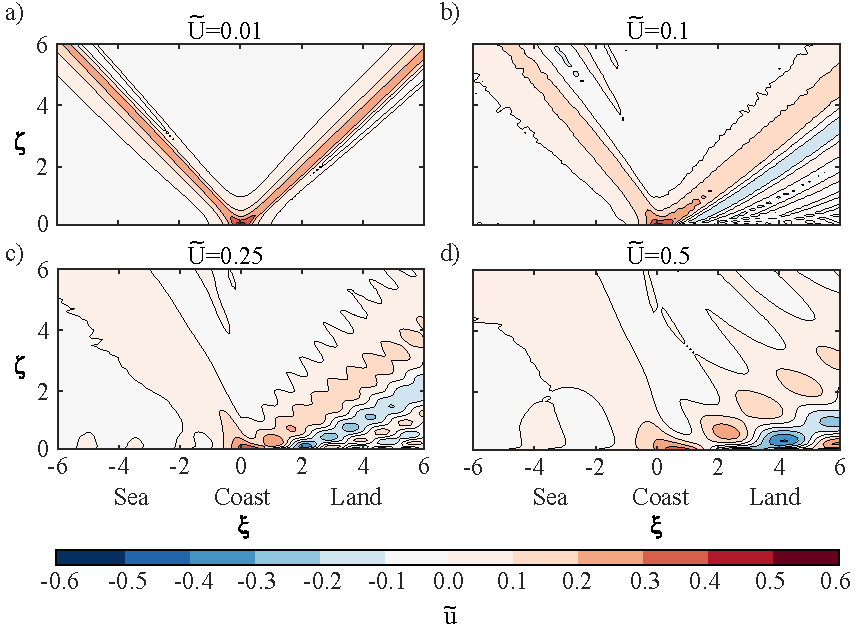
\includegraphics{qianOne.pdf}
\caption{Non-dimensional horizontal velocity $\widetilde{u}$ at 18:00 LST for a) $\widetilde{U}=0.01$,  b) $\widetilde{U}=0.1$, c) $\widetilde{U}=0.25$, d) $\widetilde{U}=0.5$.}
\label{Fig:QianOne}
\end{center}
\end{figure}


%----------------------------------------------------------------------------------------
% Chapter: Aims, Significance and Innovation
%----------------------------------------------------------------------------------------

\chapter{Aims, Significance and Innovation}
\label{Ch:Aims}

In this chapter, the three aims of this thesis are outlined, the significance of these aims are commented upon, and the innovative elements of the research are summarised.   

\section{Aims}
\label{Sec:Aims}
Three themes have emerged from the literature surveyed in the previous chapter. Firstly, many attempts have been made to explain the general ocean-morning land-evening pattern of precipitation in the Maritime Continent. However, different studies have suggested different mechanisms across different regions, and sometimes studies contradicted one another. For example, \citet{love11} found that precipitation propagated off the southwest coast of Sumatra with gravity waves triggered by stratiform heating, whereas \citet{wu09} found no evidence for this. Both studies relied on different models, which suggests that the processes involved are not sufficiently well understood to be modelled consistently. This implies a need for more observational work to guide future model development. While much research on the Maritime Continent has been done using TRMM and other satellite based precipitation data, little has been attempted using scatterometer surface wind observations. Therefore, the first aim of this thesis is to provide a representative picture of the average diurnal cycles of surface winds throughout the Maritime Continent and compare these to satellite precipitation data over the same time periods.         

In summary, this thesis will investigate three reseach questions.
\begin{enumerate}
\item
What are the mean behaviours of the diurnal cycles of surface winds across different parts of the Maritime Continent, and how do these relate to cycles of precipitation? In particular, what are the mean amplitudes, timings, offshore extents and propagation speeds of the land-sea breezes?    
\item
Does the WRF simulation of \citet{vincent16} accurately capture the timing and intensity of the diurnal cycle of surface winds? 
\item
How does the diurnal cycle of surface winds vary across different seasons and MJO phases? In particular, do land-sea breezes increase in intensity during inactive MJO phases, and do breezes respond to changes in background wind in accordance with the linear theory of \citet{qian09}?
\end{enumerate}

%----------------------------------------------------------------------------------------
% Chapter: Approach
%----------------------------------------------------------------------------------------

\chapter{Approach}
\label{Ch:Approach}
In this study, terabytes of satellite scatterometer and satellite precipitation radar data are obtained in a spatiotemporally sparse un-gridded form, binned and composited, then subjected to statistical analysis. In this chapter the scatterometer and radar datasets are introduced and the methods of analysis described and critically assessed.    

\section{Data}
This section describes the scatterometer, precipitation radar and WRF datasets considered in this study, and the potential issues with each.

\subsection{Satellite Scatterometers}
\label{Sec:Scatt}
Scatterometers work by emitting beams of microwave radiation from either aircraft or satellites, a portion of which is reflected off ocean capillary waves back to the scatterometer for detection. The wavelengths of the capillary waves can be inferred from wave superpositioning in the backscatter, as illustrated in figure \ref{Fig:Scatterometry}. If a beam of microwave energy with wavelength $\lambda$ hits the flat ocean surface at angle $\theta$ to the normal and capillary waves with wavelength $\lambda_B$ are present, the condition for superpositioning is \cite[]{stoffelen98}
\begin{equation}
\lambda_B=\frac{n}{2}\frac{\lambda}{\sin \theta}.
\end{equation}
Capillary waves respond almost instantaneously to the speed and direction of surface winds, and so the properties of the surface winds can be inferred from those of the capillary waves.

\begin{figure}
\begin{center}
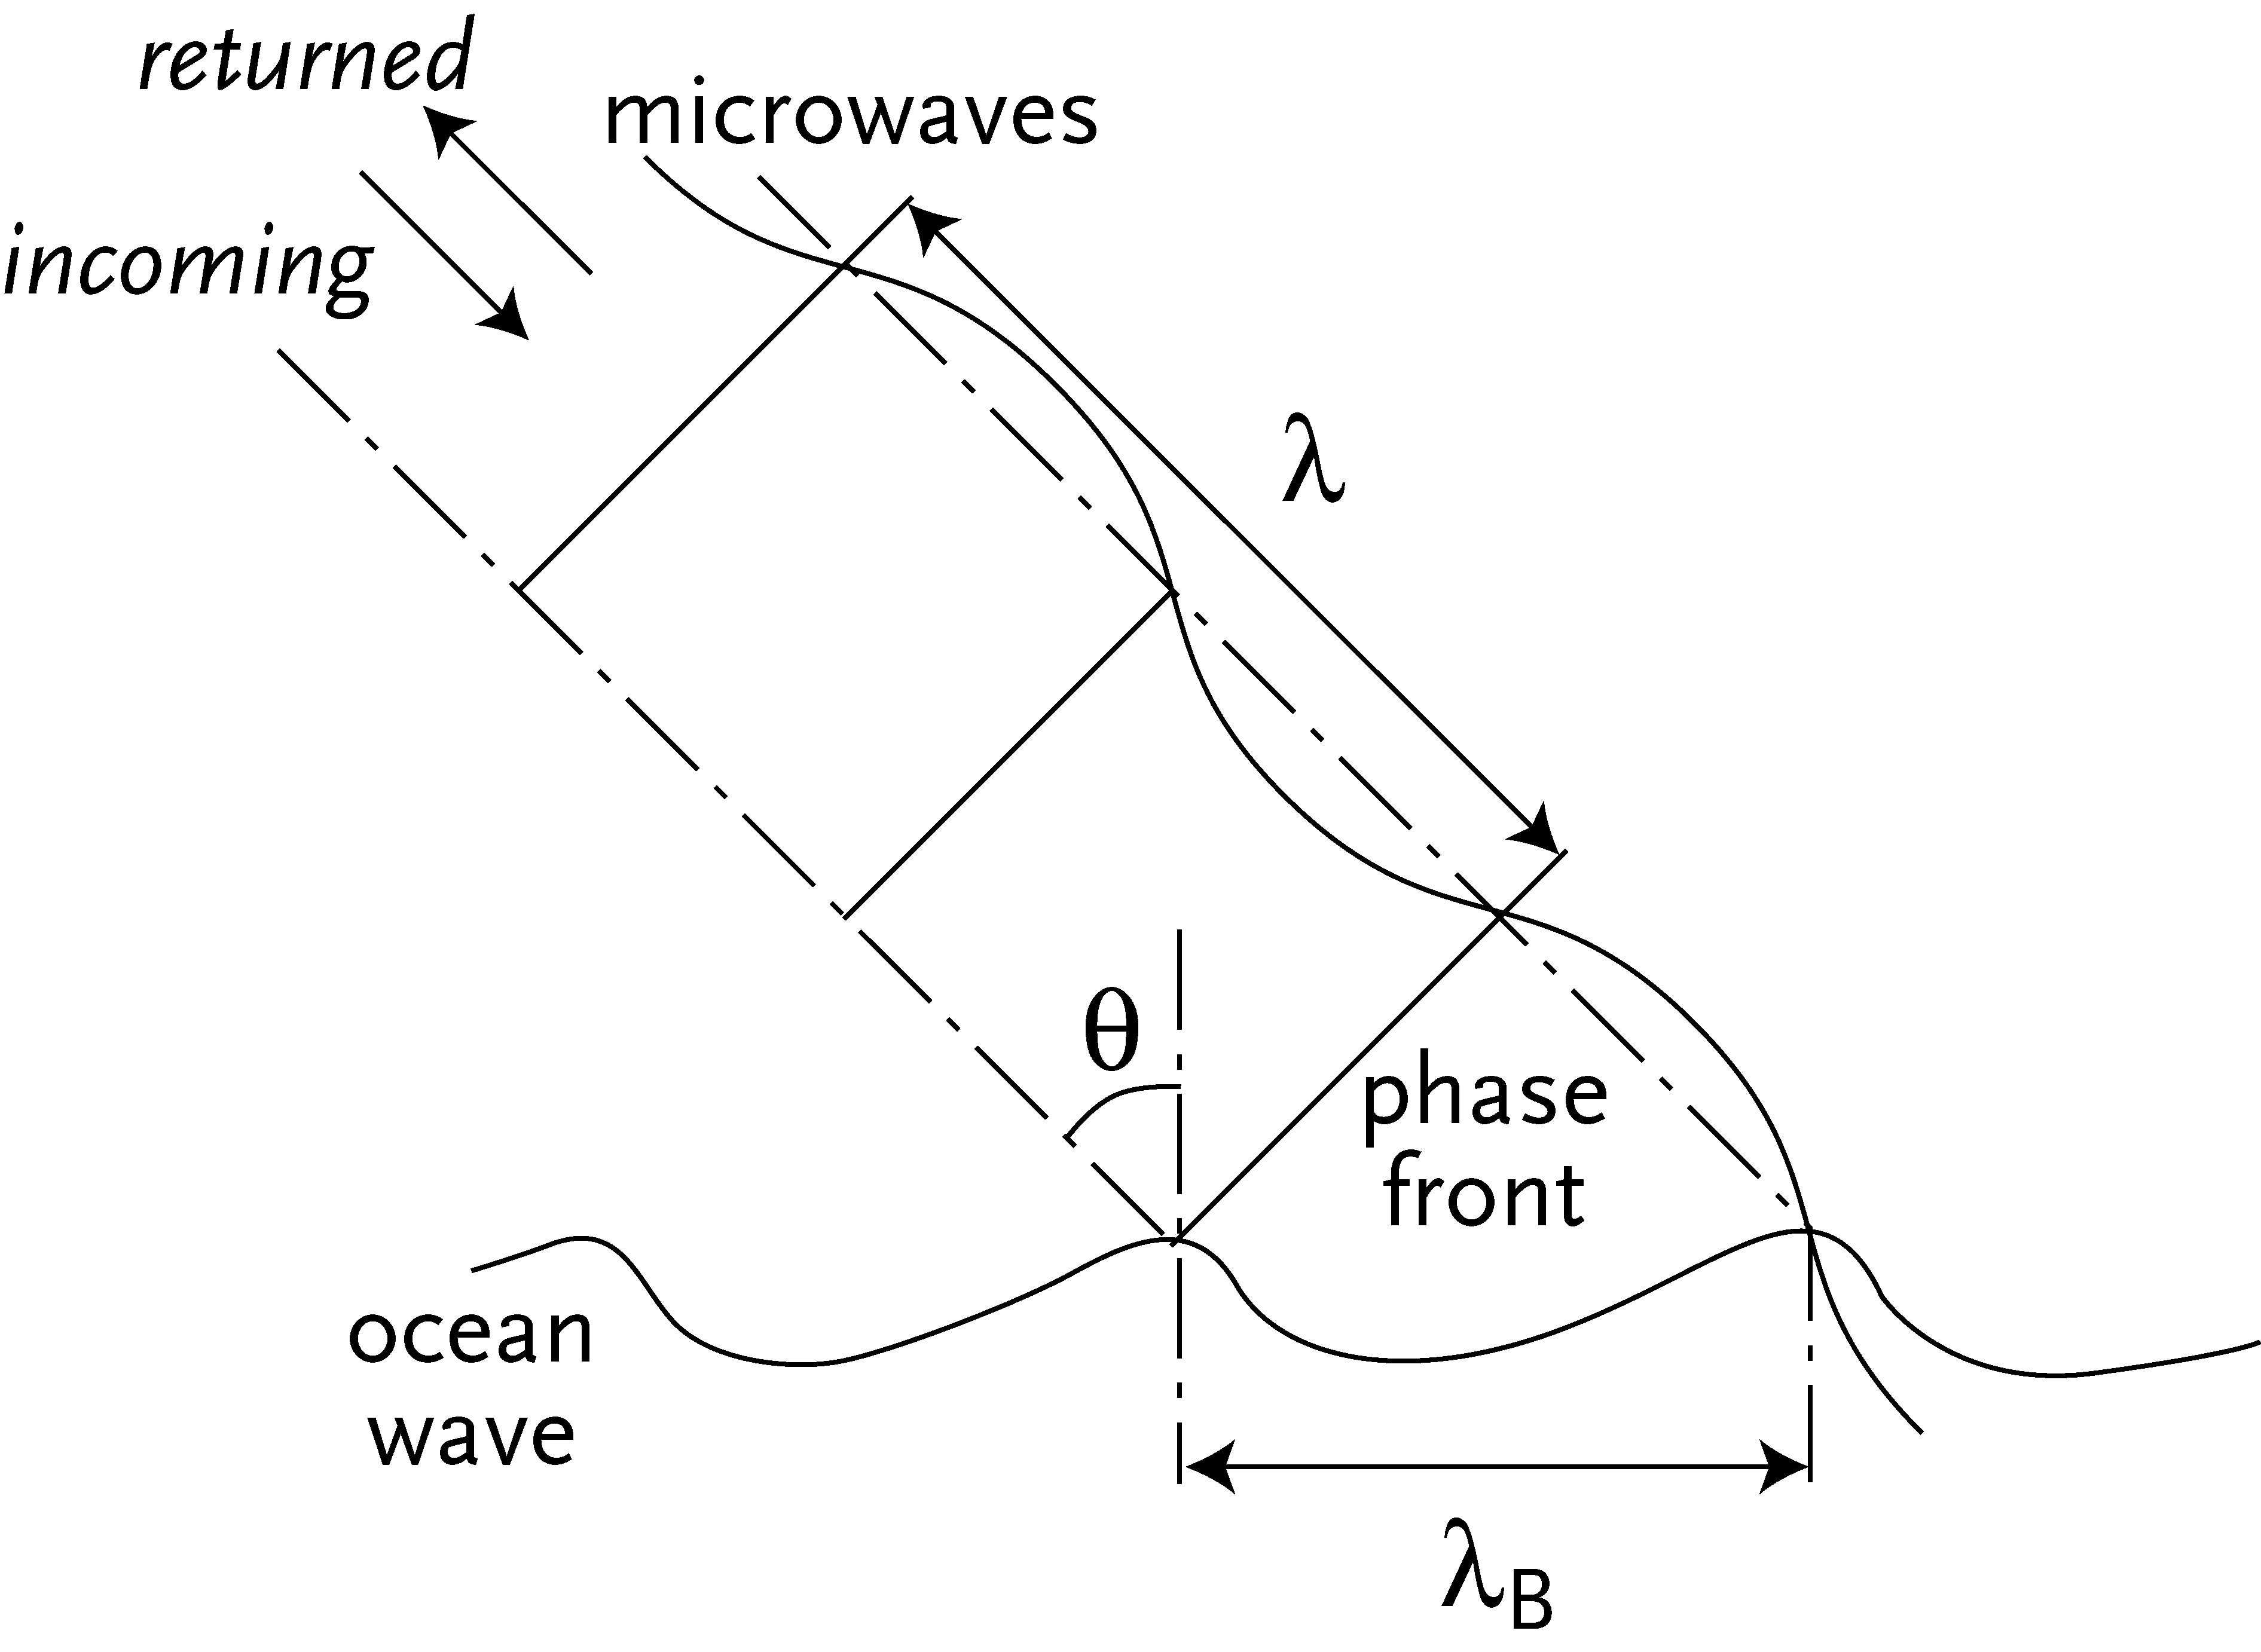
\includegraphics[scale=.07]{scatt.png}
\caption{The physical mechanism underlying scatterometry \citep[]{stoffelen98}.}
\label{Fig:Scatterometry}
\end{center}
\end{figure}

\afterpage{
\clearpage
\thispagestyle{empty}
\begin{landscape}
\centering
\begin{table} 
\begin{tabular}{ c | c | c | c | c | c | c }    
Satellite/Instrument & Frequency & Mission Duration & Pass 1 & Pass 2 & Orbit Period & Repeat Cycle \\
\hline 
Metop-A/ASCAT & 5.255 GHz & 18/08/2010 - & 08:45-10:15 & 20:45-22:15 & 101.36 min & 29 days \\
Metop-B/ASCAT & 5.255 GHz & 29/10/2012 - & 08:45-10:15 & 20:45-22:15 & 101.36 min & 29 days\\
OceanSat-2/OSCAT & 13.515 GHz & 16/01/2010 - 20/02/2014 & 10:55-12:55 & 22:55-00:55 & 99.31 min & 2 days\\
HY-2A/HY2SCAT & 13.25 GHz & 01/10/2011 - & 05:00-07:00 & 17:00-19:00 & 104.46 min & 14 days\\
ISS/RSCAT & 13.4 GHz &  03/10/2014 - 19/08/2016 & n/a & n/a & 91-93 min & n/a \\
\end{tabular}
\caption{Summary of scatterometer data availability. Pass 1 and 2 are the times in LST where each satellite samples the Maritime Continent. WRF data is available for the Austral summers between 2009-2015. ASCAT, OSCAT and HY2SCAT data overlap between 29/10/2012-20/02/2014. Data sourced from \citet[]{isro07}, \citet[]{ascat13}, \citet{moroni13}, \citet{moroni16}, \citet{nsoas13}, \citet[]{eohy17}, \citet[]{eometop17}.}
\label{Tab:satTimeInfo}
\end{table}
\end{landscape}
\clearpage
}

\begin{table} 
\begin{center}
\begin{tabular}{ c | c | c }    
Dataset & Specification & Location \\
\hline 
ASCAT & L2 12.5 km coastal & \href{podaac.jpl.nasa.gov}{podaac.jpl.nasa.gov} \\
OSCAT & L2B 12.5 km & \href{podaac.jpl.nasa.gov}{podaac.jpl.nasa.gov} \\
RSCAT & L2B 12.5 km & \href{podaac.jpl.nasa.gov}{podaac.jpl.nasa.gov} \\
HY2SCAT & L2B 25 km & \href{nsoas.gov.cn}{nsoas.gov.cn} \\
TRMM & 3G68 & \href{https://storm.pps.eosdis.nasa.gov/storm/}{storm.pps.eosdis.nasa.gov/storm/} \\
GPM & 2ADPR & \href{https://storm.pps.eosdis.nasa.gov/storm/}{storm.pps.eosdis.nasa.gov/storm/} \\
WRF & Maritime Continent v1.0 & \href{geonetwork.nci.org.au}{geonetwork.nci.org.au} \\
ERA-Interim & Top net thermal radiation & \href{http://apps.ecmwf.int/datasets/}{apps.ecmwf.int/datasets/}
\end{tabular}
\caption{Location of datasets. HY2SCAT data must be requested using a form available at \href{nsoas.gov.cn}{nsoas.gov.cn}. TRMM and GPM can be obtained by making an account with NASA's Precipitation Processing System (PPS) and using their STORM platform. A digital object identifier (DOI) for the WRF data is \href{https://geonetwork.nci.org.au/geonetwork/srv/eng/catalog.search\#/metadata/f5210\_8718\_6512\_7201}{doi:10.4225/41/5850b633c54ed}.}
\label{Tab:dataLoc}
\end{center}
\end{table}

\section{Methods}
This section explains and critically appraises the methods used in this thesis. First, the binning and compositing process is summarised, and the method for identifying the diurnally varying component of the scatterometer winds explained. Following this, the process for combining ASCAT, OSCAT and HY2SCAT data is described. Next, the method for analysing seasonal and intraseasonal variability is outlined. Lastly, the statistical tools used in this thesis are surveyed, and the use of transects discussed. 

\subsection{Binning and Compositing}
\label{Sec:Binning}
All of the scatterometer and precipitation radar data sets considered in this study are un-gridded; they provide a series of observations at $2$ to $5$ second intervals with the time, latitude and longitude at which each observation takes place. Interpreting data in this form is difficult, so each dataset is first binned into a regular longitude-latitude-time grid. The longitude, latitude and time dimension form the rows, columns and ``layers" of the grid respectively.

% Define block styles
\tikzstyle{block} = [rectangle, draw, text centered, rounded corners]
\tikzstyle{blockR} = [rectangle, draw, text centered, fill=red!10, rounded corners]
\tikzstyle{blockB} = [rectangle, draw, text centered, fill=blue!10, rounded corners]
\tikzstyle{line} = [draw, -latex']
\tikzstyle{empty} = [-latex']

\begin{figure}
\begin{center}
\begin{tikzpicture}[node distance = 1.5cm and 0.5cm, auto]
    % Place nodes
    \node [blockR, label={Day 1}] (1) {$u_1$};
    \node [blockB, right = of 1] (2) {\phantom{$u_2$}};
    \node [blockR, right = of 2, label={Day 2}] (3) {\phantom{$u_3$}};
    \node [blockB, right = of 3] (4) {$u_4$};
    \node [blockR, right = of 4, label={Day 3}] (5) {\phantom{$u_5$}};
    \node [blockB, right = of 5] (6) {$u_6$};
    \node [blockR, right = of 6, label={Day 4}] (7) {$u_7$};
    \node [blockB, right = of 7] (8) {\phantom{$u_8$}};
    \node [empty, right = of 8] (etc) {$\cdots$};

    \coordinate[below = of 4] (11);
    \coordinate[below = of 6] (22);

    \node [blockR, below = of 11] (c1) {$C_1$};
    \node [blockB, below = of 22] (c2) {$C_2$};

    % Draw edges
    \path [-] (1) edge (11);
    \path [-] (4) edge (22);
    \path [-] (6) edge (22);
    \path [-] (7) edge (11);
    \path [-] (etc) edge (11);
    \path [-] (etc) edge (22);

    \path [line] (11) -- node {Average} (c1);
    \path [line] (22) -- node {Average} (c2);
\end{tikzpicture}
\caption{Method for calculating composites. The $u_1,\ldots,u_7$ are wind observations across different time layers - empty boxes indicate where data does not exist. $C_1$ and $C_2$ denote the morning and evening composites respectively.}
\label{Fig:method1}
\end{center}
\end{figure}

\subsection{Defining Perturbations}
\label{Sec:FormingPerturbations}
Because diurnal cycles are the focus of this thesis, it is necessary to isolate the diurnally varying component of the scatterometer surface winds from the components varying at longer timescales. This is conceptually difficult because the data is so sparse. With a complete data set, the diurnal \textit{perturbation} in a given time layer could be defined by first calculating a daily average background wind centred on that time layer, then subtracting this from the value in that time layer. Repeating this over the entire domain would produce a dataset of perturbations which could then be composited as per section \ref{Sec:Binning}.

\begin{figure}
\begin{center}
\begin{tikzpicture}[node distance = 1.25cm and 0.5cm, auto]
    % Place nodes
    \node [blockR, label={Day 1}] (1) {$u_1$};
    \node [blockB, right = of 1] (2) {\phantom{$u_2$}};
    \node [blockR, right = of 2, label={Day 2}] (3) {\phantom{$u_3$}};
    \node [blockB, right = of 3] (4) {$u_4$};
    \node [blockR, right = of 4, label={Day 3}] (5) {\phantom{$u_5$}};
    \node [blockB, right = of 5] (6) {$u_6$};
    \node [blockR, right = of 6, label={Day 4}] (7) {$u_7$};
    \node [blockB, right = of 7] (8) {\phantom{$u_8$}};
    \node [empty, right = of 8] (etc) {$\cdots$};

    \coordinate[below = of 1] (11);
    \coordinate[below = of 4] (44);
    \coordinate[below = of 5] (55);
    \coordinate[below = of 6] (66);
    \coordinate[below = of 7] (77);
    \coordinate[below = of etc] (etc2);

    \node [block, below = of 11] (b1) {$b_1$};
    \node [block, below = of 44] (b4) {$b_4$};
    \node [block, below = of 66] (b6) {$b_6$};
    \node [block, below = of 77] (b7) {$b_7$};
    \node [below = of etc2] (etc3) {$\cdots$};

    \node [blockR, below = of b1] (p1) {$p_1$};
    \node [blockB, below = of b4] (p4) {$p_4$};
    \node [blockB, below = of b6] (p6) {$p_6$};
    \node [blockR, below = of b7] (p7) {$p_7$};
    \node [below = of etc3] (etc4) {$\cdots$};

    \coordinate [below = of p4] (P11);
    \coordinate [below = of p6] (P22);

    \node [blockR, below = of P11] (P1) {$P_1$};
    \node [blockB, below = of P22] (P2) {$P_2$};

    % Draw edges
    \path [-] (1) edge (11);
    \path [-] (4) edge (11);
    \path [-] (4) edge (44);
    \path [-] (7) edge (44);
    \path [-] (6) edge (66);
    \path [-] (7) edge (66);
    \path [-] (7) edge (77);
    \path [-] (6) edge (77);

    \path [line] (11) -- node {Average} (b1);
    \path [line] (44) -- (b4);
    \path [line] (66) -- (b6);
    \path [line] (77) -- (b7); 

    \path [line] (b1) -- node {Take $b_1$ from $u_1$} (p1);
    \path [line] (b4) -- (p4);
    \path [line] (b6) -- (p6);
    \path [line] (b7) -- (p7);

    \path [-] (p1) edge (P11);
    \path [-] (p7) edge (P11);
    \path [-] (etc4) edge (P11);
    \path [-] (p4) edge (P22);
    \path [-] (p6) edge (P22);
    \path [-] (etc4) edge (P22);

    \path [line] (P11) -- node {Average} (P1);
    \path [line] (P22) -- (P2);

\end{tikzpicture}
\caption{As in figure \ref{Fig:method1} but for the perturbation composites. The $b_1,\ldots,b_7$ and $p_1,\ldots,p_7$ are the background winds and perturbations respectively. $P_1$ and $P_2$ denote the perturbation composites.}
\label{Fig:method2}
\end{center}
\end{figure}

%--------------------------------------------------------------------------------------------------
% Chapter 4: Results
%--------------------------------------------------------------------------------------------------

\chapter{Results}
\label{Ch:Results}
In this chapter, the results obtained from the methods described in chapter \ref{Ch:Approach} are presented. First, section \ref{Sec:ModelComparison} provides a comparison between ASCAT and WRF over the three austral summers between 2012 and 2015. These summers represent the days common to both the WRF and ASCAT data sets. However, as discussed in the previous chapter, the diurnal cycle cannot be resolved from a single sun-synchronous data set. Furthermore, these datasets impose an unphysical symmetry on perturbation composites, which confounds the interpretation of the results.  

%--------------------------------------------------------------------------------------------------
% Chapter 5: Discussion
%--------------------------------------------------------------------------------------------------

\chapter{Discussion}
\label{Ch:Discussion}

Recall from section \ref{Sec:Aims} that this thesis has three aims. 
\begin{enumerate}
\item
Determine the mean diurnal cycle of surface winds throughout the Maritime Continent in order to better understand the mechanisms of the diurnal cycle of precipitation. 
\item
Assess the accuracy of the diurnal cycle of surface winds in the \citet{vincent16b} WRF simulation.
\item
Investigate seasonal and intraseasonal variability of the diurnal cycle of surface winds.     
\end{enumerate}
Here, the results presented in chapter \ref{Ch:Results} are discussed with reference to these aims and the literature surveyed in chapter \ref{Ch:Background}.

\begin{table} 
\begin{center}
\begin{tabular}{ | c | c | c | c | c | c |}
\hline    
Region & Dataset & L. Breeze & S. Breeze & $c_1$ & $c_2$ \\
\hline 
Sumatra & 
\begin{tabular}{@{}c@{}} RSCAT \\ CSCAT \end{tabular} & 
\begin{tabular}{@{}c@{}} 1.4 m s$^{-1}$ \\ 1.2 m s$^{-1}$ \end{tabular} & 
\begin{tabular}{@{}c@{}} -1.2 m s$^{-1}$ \\ -1.1 m s$^{-1}$ \end{tabular} & 
%\begin{tabular}{@{}c@{}} -0.3 m s$^{-1}$ \\ 0.2 m s$^{-1}$ \end{tabular} & 
\begin{tabular}{@{}c@{}} 10 m s$^{-1}$ \\ 10 m s$^{-1}$ \end{tabular} & 
\begin{tabular}{@{}c@{}} 30 m s$^{-1}$ \\ 30 m s$^{-1}$ \end{tabular} \\
\hline
South Java & 
\begin{tabular}{@{}c@{}} RSCAT \\ CSCAT \end{tabular} & 
\begin{tabular}{@{}c@{}} 0.7 m s$^{-1}$ \\ 0.5 m s$^{-1}$ \end{tabular} & 
\begin{tabular}{@{}c@{}} -0.9 m s$^{-1}$ \\ -0.6 m s$^{-1}$ \end{tabular} & 
%\begin{tabular}{@{}c@{}} -1.2 m s$^{-1}$ \\ -0.9 m s$^{-1}$ \end{tabular} & 
\begin{tabular}{@{}c@{}} 10 m s$^{-1}$ \\ 10 m s$^{-1}$ \end{tabular} & 
\begin{tabular}{@{}c@{}} 30 m s$^{-1}$  \\ 30 m s$^{-1}$ \end{tabular} \\
\hline
North Java & 
\begin{tabular}{@{}c@{}} RSCAT \\ CSCAT \end{tabular} & 
\begin{tabular}{@{}c@{}} 1.5 m s$^{-1}$ \\ 1.4 m s$^{-1}$ \end{tabular} & 
\begin{tabular}{@{}c@{}} -1.3 m s$^{-1}$\\ -1.7 m s$^{-1}$ \end{tabular} & 
%\begin{tabular}{@{}c@{}} 0.0 m s$^{-1}$ \\ 0.2 m s$^{-1}$ \end{tabular} & 
\begin{tabular}{@{}c@{}} - \\ - \end{tabular} & 
\begin{tabular}{@{}c@{}} 30 m s$^{-1}$ \\ 25 m s$^{-1}$ \end{tabular} \\
\hline
South Borneo & 
\begin{tabular}{@{}c@{}} RSCAT \\ CSCAT \end{tabular} & 
\begin{tabular}{@{}c@{}} 1.2 m s$^{-1}$ \\ 1.0 m s$^{-1}$ \end{tabular} & 
\begin{tabular}{@{}c@{}} -1.3 m s$^{-1}$ \\ -0.9 m s$^{-1}$ \end{tabular} & 
%\begin{tabular}{@{}c@{}} -1.3 m s$^{-1}$ \\ 0.8 m s$^{-1}$ \end{tabular} & 
\begin{tabular}{@{}c@{}} 5 m s$^{-1}$ \\ - \end{tabular} & 
\begin{tabular}{@{}c@{}} 25 m s$^{-1}$ \\ 25 m s$^{-1}$ \end{tabular}\\
\hline
New Guinea & 
\begin{tabular}{@{}c@{}} RSCAT \\ CSCAT \end{tabular} & 
\begin{tabular}{@{}c@{}} 1.1 m s$^{-1}$ \\ 0.9 m s$^{-1}$ \end{tabular} & 
\begin{tabular}{@{}c@{}} -1.1 m s$^{-1}$ \\ -1.0 m s$^{-1}$ \end{tabular} & 
%\begin{tabular}{@{}c@{}} -0.6 m s$^{-1}$ \\ -0.2 m s$^{-1}$ \end{tabular} & 
\begin{tabular}{@{}c@{}} 10 m s$^{-1}$ \\ 15 m s$^{-1}$ \end{tabular} & 
\begin{tabular}{@{}c@{}} 30 m s$^{-1}$ \\ 50 m s$^{-1}$ \end{tabular} \\
\hline
\end{tabular}
\caption{Summary of the perturbation and background wind speeds over each set of transects. Positive speeds indicate a wind blowing away from coastlines (land-breeze direction), negative speeds indicate a wind blowing towards coastlines (sea-breeze direction). Also shown are the propagation speeds of the land-sea breeze signal rounded to the nearest $5$ m s$^{-1}$, with $c_1$ the slower speeds close to the coastlines, and $c_2$ the faster speeds further offshore. Note that $c_1$ is generally only detectable for the land-breeze.}
\label{Tab:pertData}
\end{center}
\end{table}

\chapter{Conclusion}
\label{ch:Conclusion}

The three aims of this thesis have been addressed as thoroughly as possible, given the limitations of the datasets employed. The project also provides insight into how scatterometer data can be used to understand diurnal cycles, which will help inform future studies.  
\begin{enumerate}
\item
The RSCAT and CSCAT Hovm\"{o}ller diagrams presented in section \ref{Sec:diurnalCycle} provide two independent estimates of the diurnal cycle of surface winds near straight coastlines of the Maritime Continent. Despite the inconsistent time periods and methodological differences between the datasets, both agree on timing to within $2$ hours, and amplitude to within $0.2$ m s$^{-1}$. Across the four sets of transects studied, land-sea breeze processes are evident $400$-$600$ km offshore, with an open ocean diurnal cycle detectable $400-800$ km offshore in the case of Sumatra. Incorporating the diurnal cycle of precipitation using TRMM and GPM data suggests that different mechanisms likely account for the different precipitation propagation behaviours observed off each coastline. Off the southwest coast of Sumatra and the south coast of Java, the timing of the peak precipitation relative to that of the land-sea breezes suggest the mechanisms outlined in \citet{kilpatrick17} are at play. In the Java sea region, precipitation appears to propagate from both coastlines and peak over the sea. This occurs when the land breezes from the north coast of Java and the south coast of Borneo are active, suggesting surface convergence may also be playing a role in triggering new convection. Off the north coast of New Guinea, precipitation propagates at the same time as the land breeze perturbations, and at a similar speed. This suggests the mechanism of \citet{mapes03b} is active in this region, in agreement with the WRF simulations of \citet{vincent16}.  

Because scatterometer instruments only measure surface winds, they cannot be used to understand the complete three dimensional structure of the land-sea breeze and its propagation behaviour. While the results discussed above are consistent with hypotheses advanced by \citet{mapes03b}, \citet{kilpatrick17} and \citet{vincent16}, more precise tests could be conducted if the vertical structure of the diurnal wind cycle were available as well. One approach is to use reanalysis data. ERA-Interim was used by Kilpatrick et al. to this end, and the vertical structure characteristic of gravity wave propagation was evident. A higher resolution alternative for the Maritime Continent is the Bureau of Meteorology's Atmospheric high-resolution Regional Reanalysis for Australia (BARRA) 
product.\footnote{See \href{http://www.bom.gov.au/research/projects/reanalysis/}{www.bom.gov.au/research/projects/reanalysis/}.} However, it is unclear how well these reanalysis products resolve the vertical wave structure associated with the land-sea breeze. Another approach would be to use Doppler Radar situated near tropical coastlines to study the three-dimensional structure of the Doppler winds.\footnote{This suggestion was provided February 2018 by  \href{https://www.climatescience.org.au/staff/profile/RWarren}{Dr. Robert Warren} of Monash University.}

\item
The results of section \ref{Sec:ModelComparison} show with high confidence that the diurnal cycle of surface winds in the WRF simulation of \citet{vincent16b} exhibits timing and amplitude biases throughout most of the seas of the Maritime Continent: the WRF land-sea breeze perturbations initiate too early and are generally too intense. Given that convection over the land bodies of the Maritime Continent is often triggered by sea and valley breezes, an early and overly intense sea-breeze may partly explain WRF's early and overly intense diurnal precipitation cycle. However, this explaination is complicated by the fact that the intensity - and possibly even the timing - of the sea breeze is also affected by convective heating over land, with the latent heating from convection deepening and extending the solar heating of the land surface \citep{love11}. Furthermore, WRF's land-sea breeze timing and intensity biases are most pronounced around New Guinea, particularly along the Papuan Peninsula. This suggests that the biases are excacerbated by steep, high topography and complex coastlines. The effect of topography and convective heating on WRF's land-sea breeze biases could be investigated in future work through idealised WRF simulations that relate the timing and amplitude of land-sea and mountain-valley breezes to topography, resolution, coastline shape, convection and the boundary layer parametrisation scheme.

Note that it is unfortunately impossible to quantify the extent of WRF's land-sea breeze timing bias using just the results of section \ref{Sec:ModelComparison}. This means that it is also difficult to estimate amplitude biases, as the ASCAT data set only permits a comparison with WRF to be made at two times of day. A first estimate of the magnitude of these biases is provided by the comparisons between WRF, RSCAT and CSCAT in section \ref{Sec:diurnalCycle}. These comparisons suggest that the timing bias is at least two hours along the straight coastlines of Sumatra, Java and New Guinea, reaching up to five hours along the north coast of New Guinea. The amplitude bias along these coastlines is typically $\approx 1$ m s$^{-1}$, although along the north coast of New Guinea it approaches $\approx 1.5$ m s$^{-1}$. At least half these amplitude biases can be accounted for by seasonal inconsistencies between the data sets. Future work could address this inconsistency by comparing RSCAT and CSCAT to a WRF simulation run over the same time periods. Another option is to compare WRF data with observations from the recently completed YMC-Sumatra\footnote{See \href{http://www.jamstec.go.jp/ymc/IOP_YMC-Sumatra_2017.html}{www.jamstec.go.jp/ymc/IOP\_YMC-Sumatra\_2017.html}.} field campaign carried out by the Japan Agency for Marine-Earth Science and Technology (JAMSTEC), which used ship based measurements to study diurnal precipitation cycles around Sumatra and the Java Sea. This campaign is part of the international Years of the Maritime Continent (YMC) program; another affiliated campaign is the YMC Australian-Indonesian ship based observational campaign that will begin October 2019.\footnote{See \href{http://www.jamstec.go.jp/ymc/ymc_campaigns.html}{www.jamstec.go.jp/ymc/ymc\_campaigns.html}.}

\item
Section \ref{Sec:Variability} shows that seasonal and intraseasonal changes primarily affect the diurnal cycle of surface winds through changes to the mean wind state. Surface heating effects, such as those outlined by \citet{rauniyar11} and \citet{peatman14}, are only potentially important when the change in the mean background wind is less than a few m s$^{-1}$. The effect of the background wind on the diurnal cycle is qualitatively consistent with the linear theory of \citet{qian09}, although the symmetry that results from considering a single sun-synchronous dataset could be exaggerating the symmetric response of the onshore and offshore perturbations. To address this future work should use more temporally complete datasets. However, suitable observational datasets do not exist - station data are not available over ocean and field campaign observations are probably statistically inadequate - so model data would need to be used. Scatterometer observations therefore remain a powerful option, although to facilitate the study of diurnal cycles future scatterometer missions should employ multiple sun-synchronous satellites, as with the QuikScat-ADEOS II tandem mission, or use sun-asynchronous satellites, as with RSCAT and the ISS. 
\end{enumerate}

Overall, this thesis provides new evidence for the relationship between the diurnal cycles of surface winds and precipitatation. Advancing knowledge of precipitation processes is crucial to the development of better convection schemes, and ensuring convection resolving mesoscale models are behaving appropriately. A promising candidate for a new tropical convection parametrisation scheme is the Stochastic Multi-Cloud Model (SMCM), first proposed by \citet{khouider09}. The Australian Research Council Center of Excellence for Climate System Science has invested significantly in the development of this model \citep{peters13,dorrestijn15,peters17}, and recent work by \citet{bergemann17} has added a land-sea breeze parametrisation to the SMCM. An interesting direction for future research would be to examine whether the approach of \citet{bergemann17} improves model treatment of diurnal precipitation cycles, and whether adding additional detail to the land-sea breeze parametrisation leads to further gains in accuracy.

\appendix

\chapter{Land-Sea Breeze Linear Theory}
\label{Ap:Linear}
This section summarises the equations used in the linear theories of \citet{rotunno83} and \citet{qian09}. The equations of motion used by Rotunno are 
\begin{align}
\frac{\partial u}{\partial t}-fv&=-\frac{\partial \phi}{\partial x}, \\
\frac{\partial v}{\partial t}+fu&=0, \\
\frac{\partial w}{\partial t}-b&=-\frac{\partial \phi}{\partial z},\\
\frac{\partial b}{\partial t}+N^2w&=Q, \\
\frac{\partial u}{\partial x}+\frac{\partial w}{\partial z}&=0, \\
w(x,0,t)&=0.
\end{align}
The linearity of these equations result from treating the Coriolis force $f$ and Brunt-V\"{a}is\"{a}l\"{a} frequency $N$ as constants, and neglecting the advection term $u\frac{\partial u}{\partial x}$ from the material derivative $\frac{D u}{D t}=u\frac{\partial u}{\partial x}+\frac{\partial u}{\partial t}$. Potential temperature $\theta$ had been decomposed $\theta=\theta_0+\bar{\theta}(z)+\theta'(x,z,t)$, where $\theta_0$ is a constant reference potential temperature. Geopotential then has the form $\phi=c_p \theta_0 (P/P_0)^{R/c_p}$\footnote{From the definition of potential temperature and the ideal gas law we have $\frac{p}{\rho}=R\theta\left(\frac{p}{p_0}\right)^{\frac{R}{c_p}}$.} where $P$, $P_0$, $R$ and $c_p$ are the pressure, ground pressure, gas constant for air and the specific heat at constant pressure respectively. 

\citet{qian09} neglect the Coriolis force in their model, but include the effect of a background wind running perpendicular to the coast. The wind velocity perpendicular to the coast is decomposed as $U+u(x,z,t)$, where $U$ is a constant background wind. Linearity is obtained by neglecting the $u\frac{\partial u}{\partial t}$ and $\frac{\partial b}{\partial x}$ terms from their corresponding material derivatives. The resulting equations are  
\begin{align}
\frac{\partial u}{\partial t}+U\frac{\partial u}{\partial x}&=-\frac{\partial P}{\partial x}, \\
\frac{\partial v}{\partial t}&=0, \\
\frac{\partial P}{\partial z}&=b,\\
\frac{\partial b}{\partial t}+U\frac{\partial b}{\partial x}+N^2w&=Q, \\
\frac{\partial u}{\partial x}+\frac{\partial w}{\partial z}&=0, \\
w(x,0,t)&=0,
\end{align}
where $P$ is pressure. Note that horizontal velocity and bouyancy are now advected with the constant mean background wind $U$. 

\chapter{Statistics}
\section{The Hotelling $T^2$ Test}
\label{Ap:Stats}
In this section, the Hotelling $T^2$ test is described in more detail. Recall from section \ref{Sec:Stat} that the Hotelling $T^2$ test is the higher dimensional analogue of Student's $t$-test. The key advantage of the test is that takes into account the covariance between components of a multivariate data set \citep[p. 85]{rencher98}. The test considers two independent random samples of $p$ dimensional vectors $\boldsymbol{u}_{11}, \boldsymbol{u}_{12},\ldots, \boldsymbol{u}_{1n_1}$ and $\boldsymbol{u}_{21},\boldsymbol{u}_{22},\ldots,\boldsymbol{u}_{2n_2}$ from multivariate normal distributions $N_p(\boldsymbol{\mu}_1,\boldsymbol{\Sigma}_1)$ and $N_p(\boldsymbol{\mu}_2,\boldsymbol{\Sigma}_2)$, where $\boldsymbol{\mu_1},\boldsymbol{\mu_2}$ and $\boldsymbol{\Sigma}_1,\boldsymbol{\Sigma}_2$ denote the population means and covariance matrices respectively. The test produces a $p$-value for the null hypothesis $\boldsymbol{\mu}_1=\boldsymbol{\mu}_2$.

In the case where $\boldsymbol{\Sigma}_1=\boldsymbol{\Sigma}_2=\boldsymbol{\Sigma}$ an unbiased estimator for $\boldsymbol{\Sigma}$ is defined
\begin{equation}
\boldsymbol{S}_{pl}=\frac{(n_1-1)\boldsymbol{S}_1+(n_2-1)\boldsymbol{S}_2}{n_1+n_2-2},
\end{equation}
where $\bar{\boldsymbol{u}}_1$, $\bar{\boldsymbol{u}}_2$, $\boldsymbol{S}_1$, $\boldsymbol{S}_2$ denote the sample means and covariance matrices of $\boldsymbol{u}_1$ and $\boldsymbol{u}_2$. If the null hypothesis $\boldsymbol{\mu}_1=\boldsymbol{\mu}_2$ is true, then the test statistic
$$T^2=\frac{n_1n_2}{n_1+n_2}(\bar{\boldsymbol{u}}_1-\bar{\boldsymbol{u}}_2)'\boldsymbol{S}_{pl}^{-1}(\bar{\boldsymbol{u}}_1-\bar{\boldsymbol{u}}_2).$$
has a $T^2_{p,n_1+n_2-2}$ distribution. 

To provide some intuition as to what $T^2$ measures, note that the expression 
\begin{equation}
(\bar{\boldsymbol{u}}_1-\bar{\boldsymbol{u}}_2)'\boldsymbol{S}_{pl}^{-1}(\bar{\boldsymbol{u}}_1-\bar{\boldsymbol{u}}_2) \label{Eq:mahDis}
\end{equation}
can be rewritten
\begin{equation}
\sqrt{\left[\boldsymbol{S}_{pl}^{-\frac{1}{2}}(\bar{\boldsymbol{u}}_1-\bar{\boldsymbol{u}}_2)\right]\left[\boldsymbol{S}_{pl}^{-\frac{1}{2}}(\bar{\boldsymbol{u}}_1-\bar{\boldsymbol{u}}_2)\right]'}.
\end{equation}
Through matrix algebra it is possible to show
\begin{equation}
\text{cov}\left(\boldsymbol{S}_{pl}^{-\frac{1}{2}}(\bar{\boldsymbol{u}}_1-\bar{\boldsymbol{u}}_2)\right)=\boldsymbol{S}_{pl}^{-\frac{1}{2}}\boldsymbol{S}_{pl}\left(\boldsymbol{S}_{pl}^{-\frac{1}{2}}\right)'
=I_p 
\end{equation}
where $I_p$ is the $p$-dimensional identity matrix \citep[p. 77]{rencher02}. Equation \ref{Eq:mahDis} is therefore similar to the Euclidean distance between $\bar{\boldsymbol{u}}_1$ and $\bar{\boldsymbol{u}}_2$, but it also normalises the variance and decorrelates the components of each vector before taking the square root of the sum of squares. 

The case where $\boldsymbol{\Sigma}_1\ne\boldsymbol{\Sigma}_2$ is known as the \textit{multivariate Behrens-Fisher problem}. It is significantly more complicated as $T^2$ no longer has a $T^2_{p,n_1+n_2-2}$  distribution. Seven solutions to this problem are presented by \citet[]{christensen97}, and the solution of \citet[]{nel86} is described as the second most accurate, having the second most conservative approximation of the Type 1 error rate, and the second highest power. However, it is easier to implement and only slightly less accurate then the most accurate solution. This solution involves treating the $T^2$ test statistic as being approximately $T^2_{p,\nu}$ distributed, with
\begin{equation}
\nu=\frac{\text{tr}\left(\left[V_1+V_2\right]^2\right)+\left[\text{tr}\left(V_1+V_2\right)\right]^2}{(n_1-1)^{-1}\left[\text{tr}\left(V_1^2\right)+\text{tr}\left(V_1\right)^2\right] + (n_2-1)^{-1}\left[\text{tr}\left(V_2^2\right)+\text{tr}\left(V_2\right)^2\right]},
\end{equation}
where $V_1=\frac{S_1}{n_1}$, $V_2=\frac{S_2}{n_2}$ and $\text{tr}(X)$ denotes the trace of the matrix $X$. Note that when $\boldsymbol{\Sigma}_1=\boldsymbol{\Sigma}_2$ and $n_1=n_2$, $\nu=n_1+n_2-2$ and so $T^2$ has a $T^2_{p,n_1+n_2-2}$ distribution as before.

The most appropriate form of the $T^2$ test therefore depends on whether $\boldsymbol{\Sigma}_1=\boldsymbol{\Sigma}_2$. Hypothesis tests for $\boldsymbol{\Sigma}_1=\boldsymbol{\Sigma}_2$ exist \cite[p.138]{rencher98}, but these are not exact tests, and are very complex. Because it cannot be gaurenteed that $\boldsymbol{\Sigma}_1=\boldsymbol{\Sigma}_2$, the \citet{nel86} solution is used in this thesis. 

It is important to consider the assumptions underlying any statistical test. First is the assumption that the sampling is independent and random. This is technically false, as the exact time and date a particular grid cell is sampled by a given scatterometer are determined by the track of the satellite it is fixed to. If the observations in a given row and column of a binned dataset are viewed as a time series, then following \citet[p. 148]{wilks11}, one solution would be to calculate the lag-1 auto-correlation coefficient $\rho$, then reduce the sample size to an ``effective sample size" based on the value of $\rho$. However, it is unclear how this method should be implemented for multivariate hypothesis tests, and for long scatterometer data sets where the assumption that the time series is a first-order autoregressive process is not valid. Alternative methods for higher order autoregressive processes are available, but their implementation is even more difficult. This assumption is therefore ignored in this thesis. 

Second is the assumption that the data are sampled from multivariate normal distributions. Tests of multivariate normality generally fail across the spatial domain for scatterometer data sets, but the $T^2$-test is fairly robust to departures from normality. In a Monte Carlo simulation study, \citet[]{everitt79} showed that for the $\boldsymbol{\Sigma}_1=\boldsymbol{\Sigma}_2$ case, departures from normality decrease the effective significance level of the two sample $T^2$ test, which is the form of the test used in this thesis. Given that the only difference between the standard Hotelling $\boldsymbol{\Sigma}_1=\boldsymbol{\Sigma}_2$ test and the method of \citet[]{nel86} is the number of degrees of freedom of the test-statistic distribution, it will be assumed that Everitt's results also apply when the latter is used. \citet[]{nachtsheim88} extended the results of \citet[]{everitt79} to a broader class of non-normal distributions, and found that the $T^2$ method is robust whenever the underlying distribution is ``antipodally symmetric", a technical condition that is defined in the paper.

As a final note, recall that figure \ref{Fig:statMethodComparison} on page \pageref{Fig:statMethodComparison} provided a comparison between the $T^2$ and MANOVA tests. The MANOVA test assumes that the data from each group are sampled from multivariate normal distributions with equal covariance matrices $\boldsymbol{\Sigma}$, but the results are nevertheless similar to those of the \citet{nel86} $T^2$ test. This suggests that the assumptions of multivariate normality and equal covariance matrices do not significantly affect either test. 

\section{The Mann-Whitney Test}
\label{Ap:Mann}
This section provides a brief description of the Mann-Whitney test. Suppose first that two samples $X=\left\{x_1,\ldots,x_n\right\}$ and $Y=\left\{y_1,\ldots,y_m\right\}$ have been collected. Suppose $X$ and $Y$ are combined and ordered from smallest to largest, with the \textit{rank} of a datum its position in the order. Let $S_i$ denote the rank of $y_i$. The Mann-Whitney test statistic $W$ is then defined 
\begin{equation}
W=\sum_{j=1}^n S_j.
\end{equation}
To test for a difference in mean between $X$ and $Y$, the appropriate null hypothesis is then that $X$ and $Y$ come from the same distribution. The neat thing about $W$ is that its distribution depends only on the size of the samples $n,m$, not on the distributions of $X$ and $Y$. To simplify things, suppose $X$,$Y$ are sampled from continuous distributions so that ties do not occur in the order. In this case, there are $\binom{n+m}{m}$ possible distinct ranks for $y_1,\ldots,y_m$ and under the null hypothesis they are all equally likely. From this, the distribution of $W$ can be determined and $p$-values calculated. The method also generalises to the case of discrete data sets where ties can occur. What's more, as $\min{m,n}\to\infty$ the distribution of $W$ approaches normality, further simplifying the testing procedure. Further details on the Mann-Whitney test can be found in \citep[p.122]{hollander14}.

\bibliography{ewansbibli.bib}

\end{document}
